A Tabela \ref{tab:tempos_bubble} apresenta os tempos de execução, em segundos, obtidos para o Bubble Sort nos seis tamanhos de instância exigidos pelo trabalho, para cada um dos três tipos de entrada testados.

\begin{table}[htbp]
    \centering
    \begin{tabular}{|l|r|r|r|r|r|r|}
        \hline
         & 10 & 100 & 1.000 & 10.000 & 100.000 & 1.000.000 \\
        \hline
        Crescente & 0,000001 & 0,000000 & 0,000001 & 0,000007 & 0,000091 & 0,001795 \\
        \hline
        Decrescente & 0,000000 & 0,000031 & 0,003800 & 0,320914 & 33,378878 & 3329,210083 \\
        \hline
        Random & 0,000001 & 0,000022 & 0,002098 & 0,179071 & 27,737162 & - \\
        \hline
    \end{tabular}
    \caption{Tempo de execução (em segundos) do Bubble Sort por tamanho e tipo de instância}
    \label{tab:tempos_bubble}
\end{table}

O Gráfico \ref{fig:grafico_bubble} apresenta esses mesmos dados em escala linear. Assim como no Insertion Sort, a entrada crescente permanece praticamente em zero em todos os tamanhos (graças à parada antecipada do algoritmo), enquanto as entradas decrescente e randômica crescem de forma acentuada a partir de 10.000 elementos.

\begin{figure}[htbp]
    \centering
    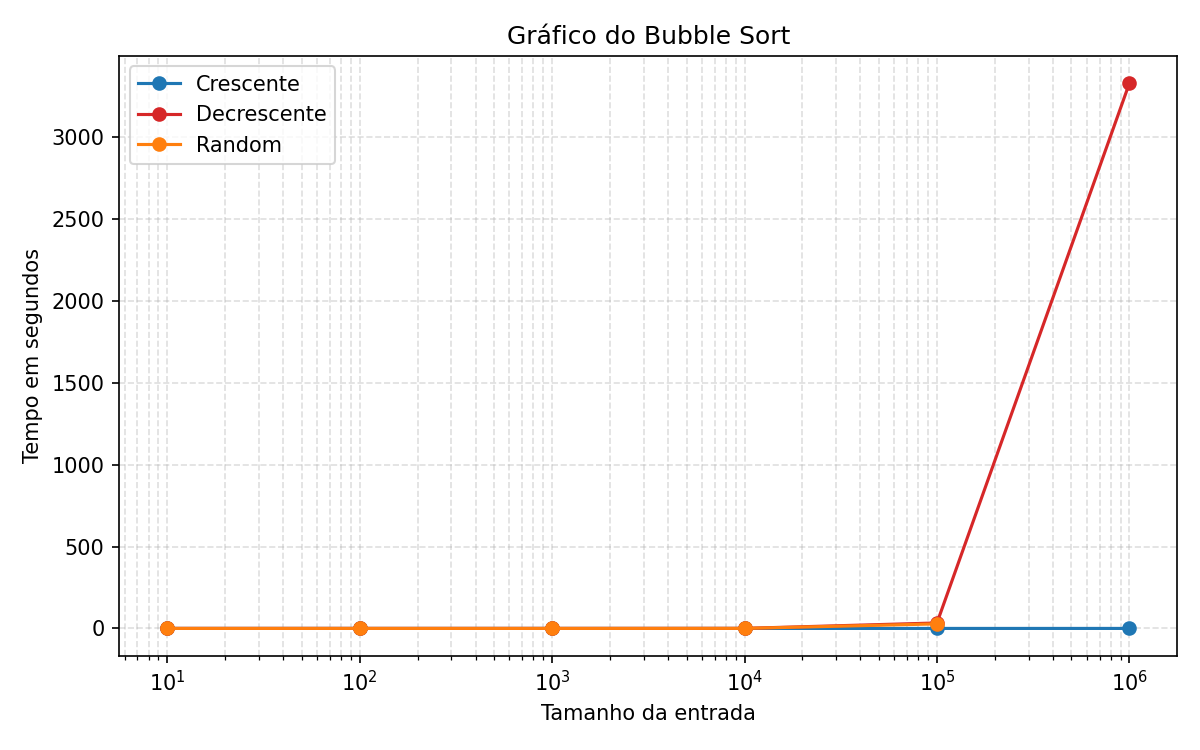
\includegraphics[width=14cm]{Imagens/Bubble Sort/grafico.png}
    \caption{Gráfico de tempo por tamanho do algoritmo Bubble Sort (escala linear)}
    \label{fig:grafico_bubble}
\end{figure}

O Gráfico \ref{fig:grafico_bubble_log} em escala logarítmica confirma o comportamento linear da entrada crescente e o comportamento quadrático das entradas decrescente e randômica. Comparando com o Insertion Sort (Capítulo 1), nota-se que o Bubble Sort é consistentemente mais lento nos casos decrescente e randômico, apesar de ambos terem a mesma ordem de grandeza de comparações -- diferença explicada pelo maior custo de cada troca do Bubble Sort (três atribuições) em comparação com o deslocamento do Insertion Sort (uma atribuição), como discutido na análise de complexidade.

\begin{figure}[htbp]
    \centering
    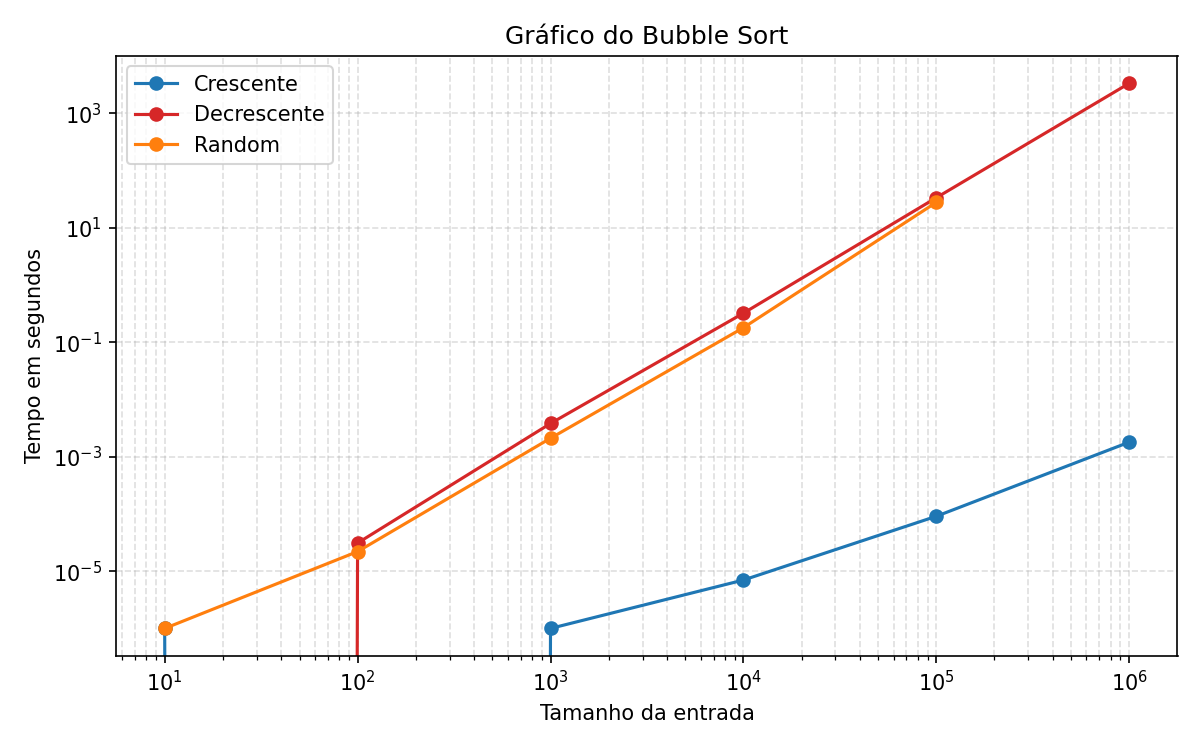
\includegraphics[width=14cm]{Imagens/Bubble Sort/grafico_log.png}
    \caption{Gráfico de tempo por tamanho do algoritmo Bubble Sort (escala logarítmica)}
    \label{fig:grafico_bubble_log}
\end{figure}
